%% -*- mode:latex; tex-open-quote:"\\og{}"; tex-close-quote:"\\fg{}" -*-
%%
%%  Copyright (c) 2002 by Pascal Vincent
%%
%%  $Id$

\documentclass[11pt]{book}
\usepackage{html}               % package for latex2html
\usepackage{t1enc}              % new font encoding  (hyphenate words w/accents)
\usepackage{ae}                 % use virtual fonts for getting good PDF
\usepackage{hyperref}
\usepackage{verbatim}

%%%%%%%%%%%%%%%%%%%%%%%%%%%%%%%%%%%%%%%%%%%%%%%%%%%%%%%%%%%%%%%%%%%%%%%%%%%%%%%
%%%  Support for PDF and required packages
%%%%%%%%%%%%%%%%%%%%%%%%%%%%%%%%%%%%%%%%%%%%%%%%%%%%%%%%%%%%%%%%%%%%%%%%%%%%%%%

\usepackage{graphicx}	% enhanced pictures import (w/ PDF)


%%% %%% Basic switch to detect whether to use PDF or not
%%% \newif\ifpdf
%%% \ifx\pdfoutput\undefined
%%%   \pdffalse
%%%   \newcommand{\mypdfoption}{{}}
%%% \else
%%%   \pdfoutput=1
%%%   \pdftrue
%%%   \newcommand{\mypdfoption}{pdftex}
%%%   \pdfcompresslevel=9
%%% \fi
%%% 
%%% %%% Packages that behave differently in PDF and non-PDF
%%% \usepackage[\mypdfoption]{graphicx}	% enhanced pictures import (w/ PDF)
%%% \usepackage[\mypdfoption]{rotating}	% rotate stuff on the page
%%% \usepackage[\mypdfoption]{color}        % color support
%%% \usepackage[\mypdfoption]{colortbl}     % Add color and shading to tables
%%% 
%%% %%% Declare graphics file extensions as .pdf or .eps for \includegraphics.
%%% %%% (You must NOT specify any extension in the filenames!  \includegraphics
%%% %%% will by itself determine the correct extension.)
%%% \ifpdf
%%%   \DeclareGraphicsExtensions{.jpg,.png,.pdf,.mps} % .png before .pdf ==> okay!
%%% \else
%%%   \DeclareGraphicsExtensions{.jpg,.eps,.png,.mps} % .eps before .png ==> okay!
%%% \fi


%%%%%%%%% Definitions %%%%%%%%%%%%
\newcommand{\R}{\sf{I\!R}} 

\newcommand{\PLearn}{{\bf \it PLearn}~}
\newcommand{\Object}{{\bf Object}~} 
\newcommand{\Learner}{{\bf Learner}~} 
\newcommand{\PPointable}{{\bf PPointable}~} 
\newcommand{\VMatrix}{{\bf VMatrix}~} 
\newcommand{\VMat}{{\bf VMat}~} 
\newcommand{\PLearner}{{\bf PLearner}~} 

\parskip=2mm
\parindent=0mm

\title{{\Huge PLearn User's Guide\\ \Large How to use the PLearn Machine-Learning library and tools}}

\begin{document}

%%%%%%%% Title Page %%%%%%%%%%
\pagenumbering{roman}

\maketitle

\vspace*{8cm}

Copyright \copyright\ 1998-2002 Pascal Vincent, Yoshua Bengio \\
Copyright \copyright\ 2002 Julien Keable \\
Copyright \copyright\ 2003 R\'ejean Ducharme \\
Copyright \copyright\ 2004 Martin Monperrus \\
Copyright \copyright\ 2005 Olivier Delalleau \\

Permission is granted to copy and distribute this document in any medium,
with or without modification, provided that the following conditions are
met:

\begin{enumerate}
\item Modified versions must give fair credit to all authors.
\item Modified versions may not be written with the aim to discredit, misrepresent, or otherwise taint the
      reputation of any of the above authors.
\item Modified versions must retain the above copyright notice, and append to
   it the names of the authors of the modifications, together with the years the
   modifications were written.
\item Modified versions must retain this list of conditions unaltered, 
    and may not impose any further restrictions.
\end{enumerate}

%%%%%%%%% Table of contents %%%%%%%%%%%%
\addcontentsline{toc}{chapter}{\numberline{}Table of contents}
\tableofcontents

% \begin{latexonly}
% \cleardoublepage\pagebreak
% \end{latexonly}
% \pagenumbering{arabic}

\pagenumbering{arabic}

%%%%%%%%%%%%%%%%%%%%%%%%%%%%%%%%%%%%%%%%%%%%%%%%%%%%%%%%%%%%%%%%%%%%%%%%%%%%%%%

\chapter*{Introduction}

PLearn is an Open Source C++ library and framework with an associated
collection of software tools developped and used for \emph{research} in
\emph{statistical machine learning.} 

The emphasis here is on \emph{``research''}: it was built by researchers
mostly for their own use, i.e. not too much with the general public in
mind. It is not for the faint of heart, and you are more likely to
find here exotic algorithms at the forefront of research, rather than a
comprehensive collection of all the ``standard proven and well tested''
algorithms of Machine Learning. This being said, if you want to program
your new idea of a learning algortihm in efficient modern C++, the PLearn
framework offers a solid foundation.

\chapter{Installation and Setup}
\label{chap:label}

\section{Requirements}

{\bf Note:} most of the tools and libraries required for PLearn are already
installed on typical Linux (or other unix-like) systems, or are easy to
install with ready-made packages (such as RPMs). PLearn is mostly
developped in a Linux environment with the gcc/g++ C++ compiler.  Since
PLearn was mostly written with portability in mind, it is certainly
portable (and has been ported on occasions) to other platforms or
compilers, but as we work mainly with Linux/gcc, we only very occasionally
check the working and correct problems on other platforms.


\subsection{Required tools}

To be able to download, compile and use PLearn, you need the following
tools to be installed on your system (for detailed instructions for
installation under Windows,
you may go directly to section~\ref{sec:windows}).
\begin{itemize}
\item {\bf g++} (http://gcc.gnu.org). We recommend using the latest version,
  but it should work with 3.2 and above. It is certainly possible to
  compile PLearn with other compilers (we do this from time to time), but
  it may necessitate some tweaking.
\item {\bf python} (http://www.python.org). Version 2.3.3 or above (may
  work with older versions, but no guarantee). We use python scripts
  heavily to make our life easier, noticeably as our compilation framework
  (but if you're really in love with Makefiles you can sure do without
  pymake).
\item {\bf subversion (svn)} for version control ( see http://subversion.tigris.org/ )
Note: some local subprojects may still be based on CVS for version control (http://www.cvshome.org)
\end{itemize}


\subsection{Libraries}

\begin{itemize}
\item {\bf required:} the standard C and C++ libraries, naturally!
\item {\bf required:} {\bf NSPR} the Netscape Portable Runtime
  (http://www.mozilla.org/projects/nspr/). We use NSPR as an OS abstraction
  layer for things such as file and network access, process control, etc...
So that PLearn may also somewhat work on Windows...
\item {\bf highly recommended:} {\bf blas} and {\bf lapack} libraries provide linear algebra
  subroutines that several learning algorithms depend upon. There are standard
  packages (RPMS\ldots) for most Linux distributions.
\item {\bf recommended:} Some learning algorithms of PLearn depend on parts
  of the {\bf boost} library (http://www.boost.org), in particular those
  requiring graph algorithms.
\item {\bf optional:} The libraries of {\bf WordNet} for work on language models.
\end{itemize}

\subsection{Useful external tools}

A number of additional tools are often used as external programs, mostly for plotting and
display purpose, and interactive GUIs, so you may want to have them installed. 
Many of them come as python modules and extensions. In particular, if you
want to empower python as a matlab-like interactive numerical manipulation
and plotting tool, you may want to install the following python packages:

\begin{itemize}
\item {\bf numarray} for efficient numeric array operations
\item {\bf matplotlib} for 2D plots (http://matplotlib.sourceforge.net/)
\item {\bf ipython} for interactive use; launch it with {\tt ipython --pylab} (http://ipython.scipy.org/) 
\item {\bf mayavi} for 3D interactive plots (http://mayavi.sourceforge.net/) built on top of VTK (http://public.kitware.com/VTK)
\item {\bf pygtk} for sophisticated GUIs.
\end{itemize}

In addition the following tools can be useful:

\begin{itemize}
\item {\bf gs} (ghostscript) and {\bf gv} (ghostview)
\item {\bf gnuplot}
\item {\bf perl} to run older dirty scripts.
\end{itemize}


\section{Downloading PLearn}

After having been hosted for several years on SourceForge (under CVS), as
of 2005/06/21 PLearn development has been moved to BerliOS
(http://developer.berlios.de/) that offered the benefits of a faster
hosting with the more modern Subversion (SVN) version control system.
The latest version is always available through SVN access.  

\subsection{Developer SVN access}
If you are going to be a serious contributor to PLearn, you should create a
BerliOS account for yourself, and ask to be added to the developer list.
This will give you read/write access to the PLearn repository.

Make sure you first move any older version of PLearn out of the way, for ex. by renaming it PLearn.old
You can then check-out a fresh copy of PLearn with the following instruction:
\begin{verbatim}
svn checkout svn+ssh://USERNAME@svn.berlios.de/svnroot/repos/plearn/trunk PLearn
\end{verbatim}
where you replace "USERNAME" by your Berlios username.
You will be asked for your Berlios password twice.

If you don't want to be bothered with svn asking passwords, clisk on {\em
  Account Maintenance} on the left panel of your BerliOS personal page, and
on {\em Edit keys} on the bottom of the Maintenance page.  You can copy
your ssh public key there. (Note: your ssh public key is normally found in
your ~/.ssh/*.pub If it's not there, you can do a ssh-keygen). As for many
changes within BerliOS, it may take a while before this is propagated and
taken into account.

We also suggest that you edit your \verb!~/.subversion/config! and look for
the line containing \verb!global-ignores!: uncomment it and add OBJS in the list
of ignored patterns, to avoid being annoyed with these directories when
doing a svn status command. You'll also have to uncomment the line
\verb![miscellany]! three lines above.

\subsection{Anonymous SVN checkout}

If you just want to hack PLearn locally, you can do an anonymous checkout (no need for a BerliOS account) with
\begin{verbatim}
svn checkout svn://svn.berlios.de/plearn/trunk PLearn
\end{verbatim}


% Sub-projects at your institution may still be under CVS.
% For a quick tutorial on how to use cvs, see http://plearn.sourceforge.net/plearncvs.html

\subsection{SVN basics}

From within your local PLearn directory:
\begin{itemize}
\item {\tt svn update} will update your local version with 
\item {\tt svn commit} will commit your changes to the repository
\item {\tt svn add} will add to the repository the files and directories
  you pass as argument, {\bf recursively}, so make sure you {\em really} want to
  add all those directories' full content\ldots
\item There is also {\tt svn rm, svn mv,} and {\tt svn cp} to reorganize the files.
\end{itemize}

Unlike CVS, most subversion commands are recursive by default. Check the
help for a particular command {\em before} using it if you are unsure.

For more details, there is a excellent free subversion book online available at:
http://svnbook.red-bean.com/en/1.1/index.html

If you don't have the time to at least peruse the whole book, I would still
strongly recommend that you at least read appendix A: Subversion for CVS
users: http://svnbook.red-bean.com/en/1.1/apa.html


\section{Initial PLearn Setup}

We suppose you have all the necessary software requirements in place (especially python).

First, edit your .cshrc or .bashrc and 
\begin{itemize}
\item Set the {\tt PLEARNDIR} environment variable to the path of your PLearn directory. 
(csh ex: \verb!setenv PLEARNDIR ${HOME}/PLearn!)
\item Append \verb!$PLEARNDIR/scripts! and \verb!$PLEARNDIR/commands! to your path.
\item Append \verb!$PLEARNDIR/python_modules! to your \verb!PYTHONPATH!
\item Restart your shell for these changes to take effect.
\end{itemize}

From within your PLearn directory run {\tt ./setup}. This should create a
{\tt .plearn} sub-directory in your home directory, that will contain some
configuration files.

Now you should be able to try and compile a first version of plearn.
We have our own make system based on a python script ({\tt pymake}) that
automatically parses source files for dependencies and determines what to
compile, and what to link (including optional libraries), and is able to
run parallel compilation on several machines.  It is easily
customizable.

The compiling commands are:
\begin{verbatim}
cd PLearn/commands/
pymake plearn_light.cc
\end{verbatim}

If it doesn't work, you may have to adapt the configuration file to your system
(PLearn/.pymake/config)

If it does work, you can try to \verb!pymake plearn.cc! (which has more dependencies on external libraries).

\section{Installing PLearn under Windows}

This section describes a step-by-step installation under the Microsoft Windows environment.

\subsection{Installation with Cygwin}

Cygwin (\url{http://cygwin.com}) is a Linux-like environment for Windows, and is
currently the easiest route to using PLearn under Windows.

\subsubsection{Installing Cygwin}

Download from \url{http://cygwin.com/setup.exe} the latest Cygwin setup program,
then run it.
Select your installation options (you should keep the recommended Unix / binary default
text file type).
Once you reach the ``Select Packages'' step, click the ``View'' button to switch
to full view and select the following packages to install (the version number in
parenthesis was the version used when this guide was written, hopefully any further
version should work too).

\begin{itemize}
\item \verb!autoconf! (2.59-2)
\item \verb!gcc-g++! (3.4.4-1)
\item \verb!gcc-g77! (3.4.4-1)
\item \verb!lapack! (3.0-3)
\item \verb!libncurses-devel! (5.4-4)
\item \verb!make! (3.80-1)
\item \verb!python! (2.4.1-1)
\item \verb!subversion! (1.2.3-1)
\end{itemize}

Optional (but recommended) packages to install:
\begin{itemize}
\item \verb!gdb! (20041228-3)
\item \verb!tcsh! (6.14.00-5)
\item \verb!unzip! (5.50-5)
\item \verb!vim! (6.4-2)
\end{itemize}

The default shell installed with Cygwin is bash, but in the following, we will
be using tcsh (though you may of course adapt the instructions below to get PLearn to
work with bash). Assuming you have installed the tcsh package and Cygwin is
installed in \verb!C:\cygwin!, edit \verb!C:\cygwin\cygwin.bat! and replace
the line \verb!bash --login -i! with \verb!tcsh -l!.
You may also change the default location of your home directory by adding the
following line at the beginning of the file (make sure you do not have blanks
in the path you provide):
\begin{verbatim}
@SET HOME=C:\MyCygwinHome
\end{verbatim}

Note that it is suggested to use a ``low-level'' path for your home directory, i.e. as close
to the root as possible, because of the limitations of Windows concerning the
length of paths (which may cause some tests to fail in the test-suite).

\subsubsection{Installing Boost}

The next step is to install the Boost library.
You could install part of it from the Cygwin setup utility, but you would
neeed to compile Boost-Python anyway.
Go to \url{http://sourceforge.net/projects/boost/} then to the ``Files'' section
to download
the Boost library. Download the \verb!tar.gz! files:
you will need the source for both Boost and Boost-Jam (the Boost installer).
Move these files to your Cygwin home directory.
The files used when writing this guide were \verb!boost_1_33_1.tar.gz!
and \verb!boost-jam-3.1.11.tgz!.

You may now run Cygwin and launch the Boost installation:
\begin{enumerate}
\item \verb!tar zxvf boost_1_33_1.tar.gz!
\item \verb!tar zxvf boost-jam-3.1.11.tgz!
\item \verb!cd boost-jam-3.1.11!
\item \verb!sh ./build.sh!
\item \verb!cd ../boost_1_33_1!
\item \verb!../boost-jam-3.1.11/bin.cygwinx86/bjam.exe -sTOOLS=gcc! \\
\verb!--prefix=$HOME/local -sPYTHON_ROOT=/usr! \\
\verb! -sPYTHON_VERSION=2.4 --builddir=/tmp/boost_build install!
\end{enumerate}

NO CYGWIN:
\begin{verbatim}
feynman ~/tmp/boost_1_33_1 > ../boost-jam-3.1.11/bin.cygwinx86/bjam.exe -sTOOLS=gcc-nocygwin --prefix=$HOME/local -sPYTHON_ROOT=R:\\python2.4_mingw -sPYTHON_VERSION=2.4 -sPYTHON_LIB_PATH=/cygdrive/r/python2.4_mingw --builddir=/tmp/boost_build_nocygwin install
\end{verbatim}

WARNING! It deletes the old libraries that were compiled with cygwin! => you cannot 'easily' have both.
NOTE: need to keep old Cygwin Python so that python scripts (e.g. pymake) work.
LAPACK INSTALL (SUX)
UNINSTALL LAPACK + .cshrc (+ autres?)
PDCURSES... FAUT EDITER LE pymake.config.model A LA MAIN POUR SWITCH PDCURSES / NCURSES (BEURK)
NE PAS OUBLIER DE COMPILER PDCURSES AVEC -mno-cygwin (a rajouter a deux endroits!)

UGLY!
\begin{verbatim}
/cygdrive/r/python2.4_mingw/include
\end{verbatim}

The installation command above will install Boost in the \verb!local! directory
under your home directory: you may remove the \verb!--prefix! option to perform
a system-wide installation (however, installing under your home directory is often
necessary for Linux users without administrator rights).
Do not worry about some of the Boost libraries not compiling, PLearn does not
need all of them.
Let us just create the appropriate links for those needed by PLearn:
\begin{enumerate}
\item \verb!cd ~/local/lib!
\item \verb!ln -s libboost_regex-gcc-mt-1_33_1.dll libboost_regex.dll!
\item \verb!ln -s libboost_python-gcc-mt-1_33_1.dll libboost_python.dll!
\item \verb!cd ~/local/include!
\item \verb!ln -s boost-1_33_1/boost!
\end{enumerate}

\subsubsection{Installing NumArray}

Download NumArray from \\
\url{http://www.stsci.edu/resources/software_hardware/numarray} \\
then install it with the following commands:
\begin{verbatim}
tar zxvf numarray-1.5.0.tar.gz
cd numarray-1.5.0
python setup.py config install --gencode --prefix=$HOME/local
\end{verbatim}

Note that (at least in version 1.5.0) there is a typo in a NumArray C++ file.
After you have installed NumArray with the commands above, edit
\verb!~/local/include/python2.4/numarray/arraybase.h! to manually remove the comma
at the end of line 117. Additionally, if you want to get rid of a gcc warning
when compiling PLearn, you can edit \verb!libnumarray.h!
in the same directory and replace line 51 with
\begin{verbatim}
static void **libnumarray_API __attribute__ ((unused)) ;
\end{verbatim}

\subsubsection{Installing NSPR}

Go to \verb!ftp://ftp.mozilla.org/pub/mozilla.org/nspr/releases! to get
the NSPR release for your operating system (in this guide we used the
4.6 release for Windows NT 5.0, in optimized mode).
Extract the zip file to a temporary directory, then move the content of the
\verb!include! directory (including its sub-directories) to \verb!~/local/include/mozilla/nspr! (that you
will need to create), and the
\verb!libnspr4.dll! file (in the \verb!lib! directory) to \verb!~/local/lib!.
Check the permissions for \verb!libnspr4.dll!: you need the ``execute'' permission
for PLearn to be able to run. You can set it with:\\
\verb!chmod u+x ~/local/lib/libnspr4.dll!

\subsubsection{Installing PLearn}

You are now ready (at last!) to install PLearn. First, go to the directory
where you wish to install PLearn (in this guide we will assume this is your
home directory), and check out the latest
version from the Subversion repository:\\
\verb!svn checkout svn://svn.berlios.de/plearn/trunk PLearn!

Since \verb!pymake! will create directories named \verb!OBJS! to store
compiled object files, Subversion should ignore them: edit
your \verb!~/.subversion/config! and, in the \verb!miscellany! section,
write the line\\
\verb!global-ignores = OBJS!

Now, edit your \verb!~/.cshrc! and add the following lines:

\begin{verbatim}
# Environment variables.
setenv PLEARNDIR ${HOME}/PLearn
setenv PATH /usr/local/bin:/usr/bin:/bin:/usr/lib/lapack:
            ${PLEARNDIR}/commands:${PLEARNDIR}/scripts:
            ${HOME}/local/lib
setenv PYTHONPATH ${PLEARNDIR}/python_modules:
                  ${HOME}/local/lib/python2.4/site-packages
setenv CPATH ${HOME}/local/include
setenv LD_LIBRARY_PATH ${HOME}/local/lib
setenv LIBRARY_PATH ${LD_LIBRARY_PATH}

# Nicer prompt.
set prompt = "%B%m %~%b > "
\end{verbatim}

You need to redefine the \verb!PATH! environment variable because the
original one will usually contain directories with blanks (such as
\verb!Program Files!), which Cygwin has trouble with.
The last line is very optional (it just gives you a nicer prompt).
Now edit \verb!$PLEARNDIR/pymake.config.model! and look for the
\verb!python! optional library.
Just before, add the following lines:
\begin{verbatim}
python_version = '2.4'
compileflags += ' -DPL_PYTHON_VERSION=240'
python_lib_root = '/usr/lib'
numpy_site_packages = join(homedir,
              'local/lib/python2.4/site-packages/numarray')
\end{verbatim}

Do a \verb!source ~/.cshrc! to reload your configuration file, then go
to your PLearn installation directory (\verb!$PLEARNDIR!) and run \verb!./setup!. PLearn can now be compiled
with \verb!pymake $PLEARNDIR/commands/plearn!.

\subsubsection{Testing PLearn}

Once PLearn compiles successfully, it is recommended to run the test-suite
in order to ensure that the main components of the library work as expected.
Go to \verb!$PLEARNDIR! and launch \verb!pytest run --all!.
Note that, typically, the test-suite first compiles \verb!$PLEARNDIR/commands/plearn_tests!,
and thus may look like it is stalled, while it is actually compiling or linking
in the background.

\subsection{Installation with MinGW}

- MSys MSYS-1.0.10.exe from http://www.mingw.org/ then Download
- msys.bat:
@set PATH=R:\msys\bin
@set HOME=R:\msys\home
- uncompress mingw-runtime-3.9.tar.gz
- uncompress gcc-core-3.4.2-20040916-1.tar.gz
- uncompress gcc-g++-3.4.2-20040916-1.tar.gz
- uncompress binutils-2.15.91-20040904-1.tar.gz
- uncompress w32api-3.5
- rajouter /etc/fstab contenant R:/mingw /mingw
- download de python-2.4.2.msi pour installation Python
- download de http://starship.python.net/crew/kernr/mingw32/pexports-0.42h.zip
=> pexports.exe dans /r/mingw/bin



- NO : Subversion : svn-win32-1.2.3.zip from http://subversion.tigris.org/servlets/ProjectDocumentList?folderID=91
- subversion-1.1.4.tar.gz from http://subversion.tigris.org/servlets/ProjectDocumentList?folderID=260&expandFolder=74
tar zxvf subversion-1.1.4.tar.gz
cd subversion-1.1.4
./configure
=> IMPOSSIBLE DE FAIRE FONCTIONNER SVN SOUS MINGW !!
=> UTILISER CYGWIN ?...

\chapter{Overview of the directory structure}

Your checked out PLearn has the following high level directory structure:

\begin{itemize}
\item \verb!scripts/! \\
contains mostly python and perl scripts
  \begin{itemize}
  \item {\tt pymake} is our build system 
  \item {\tt pytest} implements our test suite framework
  \item {\tt pyskeleton} is our ``wizard'' or ``template'' system;  it uses source code templates in the {\tt Skeleton/} directory
  \item {\tt pypoints} allows graphical interactive input of points (for 2D classif or 1D regression)
  \item {\tt pyplot} allows plotting learner outputs (classif decision surface, density plot, etc...) 
  \item {\tt xpdir} lists the content of PLearn experiment directories
  \item {\tt perlgrep}, {\tt search-replace}, and {\tt undo-search-replace} allow for simple code lookup and transformations.
  \item {\tt pytansform} and the transformations in {\tt Transformations/} allow for complex code transformations.
  \item {\tt cvschangeroot} is used to recursively change the locally recorded cvs root. This is useful to indicate that the repository has moved.
  \item \ldots
  \end{itemize}
\item \verb!commands/! \\ 
contains the main plearn programs (as {\tt .cc} files that can be compiled with {\tt pymake})
  \begin{itemize}
  \item \verb!plearn_light.cc! is a minimalistic plearn with limited dependencies
    on external libraries
  \item \verb!plearn.cc! is a full plearn with a lot of algorithms
    compiled in (with more dependencies on external libraries)
  \item \verb!PLearnCommands/! contains the source code for all PLearn
    commands (these commands are included in \verb!plearn.cc! or \verb!plearn_light.cc!)
  \item \verb!language/! contains some programs for manipulating language
    corpus and WordNet related stuff.
  \end{itemize}
\item \verb!python_modules/! \\
The root for python module namespace. Must be in your \verb!PYTHONPATH!. \\
It contains mostly a \verb!plearn/! subdirectory, which allows to \verb!import plearn.foobar! from python.
\item \verb!doc/! \\
directory within which Pearn's documentation is generated
\item \verb!examples/! \\
contains examples of PLearn scripts 
\item \verb!test_suite! \\
contains part of the PLearn test suite
\item \verb!plearn/! \\
contains all of PLearn's base C++ classes organised in themed subdirectories.
\item \verb!plearn_learners/! \\
contains all of PLearn's C++ learner classes organised in themed subdirectories.
\item \verb!plearn_learners_experimental/! \\
may contain some {\em very experimental} C++ learner classes\ldots
\item \verb!plearn_torch/! \\
contains C++ classes to interface with the Torch library ( http://www.torch.ch/ )
\item \verb!pylearn/! \\
is the beginning of a BoostPython interface to access PLearn from python
\end{itemize}

The \verb!plearn*! directories contain C++ source code ({\tt .h} and {\tt
  .cc}), and as your root PLearn directory is in the \verb!-I! directive of
the compilation commands, this allows to include relevant files by
directives such as, for ex:
\begin{verbatim}
#include<plearn/base/Object.h>
#include<plearn/io/PStream.h>
#include<plearn_learners/generic/PLearner.h>
\end{verbatim}


\chapter{Tutorial}

This chapter is a tutorial that will walk you through the basic concepts from a user-level perspective.

We assume you have a copy of the plearn distribution, and a working plearn
executable accessible through yout PATH. All the files in this tutorial are in \verb!examples/Tutorial/!
so you should first {\tt cd} to this directory.

\section{The plearn Commands and Help}

Usual PLearn executables such as \verb!plearn! or \verb!plearn_light! are
typically called in command-line fashion.

\begin{verbatim}
valhalla:~/PLearn/examples/Tutorial> plearn
plearn 0.92.0  (Jun 21 2005 12:04:50)
Type 'plearn help' for help


valhalla:~/PLearn/examples/Tutorial> plearn help
plearn 0.92.0  (Jun 21 2005 12:04:50)
To run a .plearn script type:                       plearn scriptfile.plearn
To run a command type:                              plearn command [ command arguments ]

To get help on the script file format:              plearn help scripts
To get a short description of available commands:   plearn help commands
To get detailed help on a specific command:         plearn help <command_name>
To get help on a specific PLearn object:            plearn help <object_type_name>
To get help on datasets:                            plearn help datasets
\end{verbatim}

The {\tt plearn} executable can be invoked either with a {\em PLearn script} (more on that later) or with a {\em PLearn command}.\\
To get the list of available commands:

\begin{verbatim}
valhalla:~/PLearn/examples/Tutorial> plearn help commands
plearn 0.92.0  (Jun 21 2005 12:04:50)
To run a command, type:  % plearn command_name command_arguments

Available commands are:
FieldConvert    :  Reads a dataset and generates a .vmat file based on the data, but optimized for training.

autorun :  watches files for changes and reruns the .plearn script
help    :  plearn command-line help
htmlhelp        :  Output HTML-formatted help for PLearn
jdate   :  Convert a Julian Date into a JJ/MM/YYYY date
ks-stat :  Computes the Kolmogorov-Smirnov statistic between 2 matrix columns
learner :  Allows to train, use and test a learner
read_and_write  :  Used to check (debug) the serialization system
run     :  runs a .plearn script
server  :  Launches plearn in computation server mode
test-dependencies       :  Compute dependency statistics between input and target variables.
test-dependency :  Compute dependency statistics between two selected columns of a vmat.
vmat    :  Examination and manipulation of vmat datasets


For more details on a specific command, type:
  % plearn help <command_name>

\end{verbatim}

PLearn commands accept a number of arguments that are command specific.
Very often the first argument is itself a sub-command\ldots

{\tt help} is actually a {\em PLearn command}! Thus we can ask help on help!

\begin{verbatim}
valhalla:~/PLearn/examples/Tutorial> plearn help help
plearn 0.92.0  (Jun 21 2005 12:04:50)
*** Help for command 'help' ***
plearn command-line help
help <topic>
Run the help command with no argument to get an overview of the system.
\end{verbatim}

The {\tt help} command can give detailed help on any available PLearn {\em
  command}, as well as on any PLearn {\em object class}.

{\bf There is an on-line html version of the help provided by the help command...}
See {\em PLearn help on user-level commands and objects} on the PLearn homepage\ldots

\section{Data Matrices}

Machine-learning algorithms learn from data and are then used for prediction on new data.
In this tutorial, we'll concentrate on the simplest and most usual form of
data samples: vectors in $\R^d$. 

A dataset of $l$ samples is then simply an $l \times d$ matrix of reals.
In PLearn such datasets are implemented through the concept of a \VMatrix
(or \VMat in short).

A \VMat is essentially:
\begin{itemize}
\item A $l \times d$ matrix of reals ($l$ is its {\em length}, $d$ its {\em width}),
\item optionally with an associated {\em fieldname} for each column (or {\em field}),
\item optionally with associated {\em inputsize, targetsize, weightsize}
\item optionally with strings associated to specific values of a given column
\end{itemize}

The {\em inputsize, targetsize, weightsize} are important information for
learning algorithms, as they specify which part of each row is to be
considered the known input (the first {\em inputsize} elements), which part
is the target to predict (the next {\em targetsize} elements), and whether
or not they are followed by a sample weight ({\em weightsize = 0 or
  1}).

For the traditional {\em tasks} of statistical machine learning, we have
the following conventions regarding datasets and ``sizes'':
\begin{itemize}
\item {\bf regression:} \\
{\em inputsize} = number of known inputs (``variables'', ``factors'' or ``features'', i.e. dimensioality of ``$x$'')\\
{\em targetsize} = number of values to predict (i.e. dimensionality of ``$y$'')
\item {\bf classification:} \\
{\em inputsize} = number of known inputs \\
{\em targetsize} = 1: the target is the class number (between 0 and nclasses-1)
\item {\bf density estimation:} \\
{\em inputsize} = dimensionality of $x$ \\
{\em targetsize} = 0
\end{itemize}


For ex., let's create a simple data set for 1D regression, i.e. to predict a real $y$ from a real $x$.
Open a file \verb!1d_reg.amat! with your favorite editor, and and enter the following text definint a 
$5 \times 2$ matrix:
\begin{verbatim}
#size: 5 2
#: x y     
#sizes: 1 1 0

0    3
0.5  4
1    5
2    6
3    7.5
\end{verbatim}

This represents a $5 \times 2$ matrix whose columns are named {\em x} and
{\em y}, and whose {\em inputsize=1, targetsize=1, weightsize=0}.

\section{Viewing Data Matrices}

Data matrices can be manipulated with the PLearn command {\em vmat}:

\begin{verbatim}
valhalla:~/PLearn/examples/Tutorial> plearn help vmat
plearn 0.92.0  (Jun 21 2005 12:04:50)
*** Help for command 'vmat' ***
Examination and manipulation of vmat datasets
Usage: vmat info <dataset>
       Will info about dataset (size, etc..)
   or: vmat fields <dataset> [name_only] [transpose]
       To list the fields with their names (if 'name_only' is specified, the indexes won't be displayed,
       and if 'transpose' is also added, the fields will be listed on a single line)
   or: vmat fieldinfo <dataset> <fieldname_or_num> [--bin]
       To display statistics for that field
   or: vmat bbox <dataset> [<extra_percent>]
       To display the data bounding box (i.e., for each field, its min and max, possibly extended by +-extra_percent ex: 0.10 for +-10% of the data range )
   or: vmat cat <dataset> [<optional_vpl_filtering_code>]
       To display the dataset
   or: vmat sascat <dataset.vmat> <dataset.txt>
       To output in <dataset.txt> the dataset in SAS-like tab-separated format with field names on the first line
   or: vmat view <dataset>
       Interactive display to browse on the data.
   or: vmat stats <dataset>
       Will display basic statistics for each field
   or: vmat convert <source> <destination> [--cols=col1,col2,col3,...]
       To convert any dataset into a .amat, .pmat, .dmat or .csv format.
       The extension of the destination is used to determine the format you want.
       If the option --cols is specified, it requests to keep only the given columns
       (no space between the commas and the columns); columns can be given either as a
       number (zero-based) or a column name (string).  You can also specify a range,
       such as 0-18, or any combination thereof, e.g. 5,3,8-18,Date,74-85
       If .csv (Comma-Separated Value) is specified as the destination file, the
       following additional options are also supported:
         --skip-missings: if a row (after selecting the appropriate columns) contains
                          one or more missing values, it is skipped during export
         --precision=N:   a maximum of N digits is printed after the decimal point
         --delimiter=C:   use character C as the field delimiter (default = ',')
   or: vmat gendef <source> [binnum1 binnum2 ...]
       Generate stats for dataset (will put them in its associated metadatadir).
   or: vmat genvmat <source_dataset> <dest_vmat> [binned{num} | onehot{num} | normalized]
       Will generate a template .vmat file with all the fields of the source preprocessed
       with the processing you specify
   or: vmat genkfold <source_dataset> <fileprefix> <kvalue>
       Will generate <kvalue> pairs of .vmat that are splitted so they can be used for kfold trainings
       The first .vmat-pair will be named <fileprefix>_train_1.vmat (all source_dataset except the first 1/k)
       and <fileprefix>_test_1.vmat (the first 1/k of <source_dataset>
   or: vmat diff <dataset1> <dataset2> [<tolerance> [<verbose>]]
       Will report all elements that differ by more than tolerance (defauts to 1e-6).
       If verbose==0 then print only total number of differences
   or: vmat cdf <dataset> [<dataset> ...]
       To interactively display cumulative density function for each field
       along with its basic statistics
   or: vmat diststat <dataset> <inputsize>
       Will compute and output basic statistics on the euclidean distance
       between two consecutive input points

<dataset> is a parameter understandable by getDataSet:
Dataset specification can be one of:
 - the path to a matrix file (or directory) .amat .pmat .vmat .dmat or plain ascii
 - ... 
\end{verbatim}

OK, too many subcommands here, but let's concentrate on the few ones you're most likely to use:

\begin{verbatim}
valhalla:~/PLearn/examples/Tutorial> plearn vmat info 1d_reg.amat
plearn 0.92.0  (Jun 21 2005 12:04:50)
5 x 2
inputsize: 1
targetsize: 1
weightsize: 0


valhalla:~/PLearn/examples/Tutorial> plearn vmat fields 1d_reg.amat
plearn 0.92.0  (Jun 21 2005 12:04:50)
FieldNames:
0: x
1: y


valhalla:~/PLearn/examples/Tutorial> plearn vmat fieldinfo 1d_reg.amat y
plearn 0.92.0  (Jun 21 2005 12:04:50)
[------------------------------------- Computing statistics (5) -------------------------------------]
[....................................................................................................]
Field #1:  y     type: UnknownType
nmissing: 0
nnonmissing: 5
sum: 25.5
mean: 5.09999999999999964
stddev: 1.74642491965729807
min: 3
max: 7.5


valhalla:~/PLearn/examples/Tutorial> plearn vmat cat 1d_reg.amat
plearn 0.92.0  (Jun 21 2005 12:04:50)
0 3
0.5 4
1 5
2 6
3 7.5
\end{verbatim}

If you want to browse the data matrix interactively, you can use the
command \verb!plearn vmat view 1d_reg.amat! (This is most useful for huge data sets\ldots)

You can also see the points graphically by using the \verb!pyplot! script
\verb!pyplot plot_2d 1d_reg.amat!

\section{vmat File Formats}

The {\em V} in \VMatrix stands for {\em Virtual}, because \VMatrix is a C++ virtual
base class of which there are several concrete derived classes (do a
\verb!plearn help VMatrix! if you want to see how many\ldots).

Accordingly, there are several file formats that represent real data
matrices, distinguished by their file extension:

% \begin{table}[h]
% \caption{vmat file extensions and formats}
% \label{tab:vmat-formats}
\begin{center}
\begin{tabular}{|l|l|} \hline 
{\bf extension} & {\bf format description} \\ \hline
.amat           & Simple ascii format  \\ \hline
.pmat           & Simple raw binary format with 1 line ascii header  \\ \hline
.dmat           & Directory containing compressed binary data        \\
                & (possibly split in several files for huge data)    \\ \hline
.vmat           & Contains the specification of a C++ VMatrix object \\ 
                & (in PLearn's ascii serialisation format)           \\ \hline
.pymat          & Python preprocessing code that generates the       \\ 
                & specification of a C++ VMatrix object (a la .vmat) \\ \hline
\end{tabular}
\end{center}
% \end{table}

In addition, several of those tend to have an associated {\tt .metadata}
directory, that will contain associated data that is not held within the
file itself (for ex: fieldnames, inputsize and targetsize, field statistics, etc\ldots)

You can convert from any format to {\tt .amat, .pmat, .dmat, .csv} with PLearn
command {\tt vmat convert}:
\begin{verbatim}
plearn vmat convert 1d_reg.amat 1d_reg.pmat
plearn vmat view 1d_reg.pmat
\end{verbatim}

\section{PLearn Objects, Their Serialization and Specification}

PLearn is first and foremost a C++ class library. PLearn also provides a
mechanism to serialize such objects to and from files (i.e. write a
representation of an in-memory object to a file, or later reload such a
saved object from that file). PLearn serialization supports both an ASCII
human-readable format (\verb!plearn_ascii!), and a more efficient binary format (\verb!plearn_binary!).

As a result of this capability, it is also possible to {\em specify} a
PLearn object by simply writing its ASCII serialized form by hand. 
This is basically what a {\tt .vmat} file contains: {\em the ASCII serialised form of a C++ subclass of VMatrix}.

For example, create a file \verb!selected_rows.vmat! with the following content:

\begin{verbatim}
SelectRowsVMatrix(
  source = AutoVMatrix( specification = "1d_reg.amat" ),
  indices = [ 1 1 3 0 3 4],
  inputsize =   1,
  targetsize =  0,
  weightsize =  1
);
\end{verbatim}

The serialised form of most PLearn objects, as can be seen here, is:
\begin{verbatim}
ObjectName(  
  optionname = optionval
  optionname = optionval
  ...
)
\end{verbatim}

Note that in \verb!plearn_ascii! format, in general, spaces, newlines, commas and semicolons
are ignored (any sequence of those is considered a single separator).

There is typically a one to one correspondance between an object's {\em
  options} (in its serialised form) and the fields of the corresponding C++
object. A PLearn object often has many options, but they always have a default value,
so that there is no need to explicitly set those for which the default value is fine.

The above {\tt .vmat} specifies an object of type {\tt SelectRowsVMatrix},
which is a sort of vmat that will select desired rows from another
``source'' vmat.  \verb!selected_rows.vmat! will thus be an {\em altered
  view} of \verb!1d_reg.amat!, for which we also change the values of {\em
  inputsize, targetsize, weightsize}.

\begin{verbatim}
valhalla:~/PLearn/examples/Tutorial> plearn vmat info selected_rows.vmat
plearn 0.92.0  (Jun 22 2005 19:42:18)
6 x 2
inputsize: 1
targetsize: 0
weightsize: 1


valhalla:~/PLearn/examples/Tutorial> plearn vmat cat selected_rows.vmat
plearn 0.92.0  (Jun 22 2005 19:42:18)
0.5 4
0.5 4
2 6
0 3
2 6
3 7.5
\end{verbatim}

Help on any plearn object can be obtained, as usual, by invoking
\verb!plearn help ! {\em objectclass}. This will output a commented serialised object, with all its build {\em
  options} and their default value. This help is also available in online html form. For ex. try:

\begin{verbatim}
plearn help SelectRowsVMatrix
\end{verbatim}

This makes for a good starting point for writing a {\tt .vmat} (or {\tt
  .plearn}), as you can issue:
\begin{verbatim}
plearn help SelectRowsVMatrix > mymat.vmat
\end{verbatim}
and then edit the file to your liking (removing unnecessary options that
are to keep their default value, etc...)

{\tt .vmat} is not the only file extension associated with specifications
of PLearn objects in serialised form. Here are the other extensions you may
encounter:

\begin{center}
\begin{tabular}{|l|l|} \hline 
{\bf extension} & {\bf format description} \\ \hline
.vmat           & specification of a subclass of VMatrix in \verb!plearn_ascii!    \\ 
                & serialization format (with rudimentary macro-processing)  \\ \hline
.plearn         & specification of any PLearn object in \verb!plearn_ascii!        \\
                & format (with rudimentary macro-processing)                \\ \hline
.psave          & serialized PLearn object in \verb!plearn_ascii! or \verb!plearn_binary! \\
                & format (does not undergo macro-explansion)                \\ \hline
.pymat          & Python preprocessing code that generates the              \\ 
                & \verb!plearn_ascii! specification of a VMatrix subclass          \\ \hline 
.pyplearn       & Python preprocessing code that generates the              \\ 
                & \verb!plearn_ascii! specification of any PLearn object           \\ \hline
\end{tabular}
\end{center}

While {\tt .vmat} and {\tt .plearn} support some rudimentary
macro-processing, this is deprecated in favor of the power of the Python
preprocessing of {\tt .pymat} and {\tt .pyplearn} files. We will get back
to this later.

\section{plearn Learner}

The concept of a learning algorithm in PLearn is implemented through the \PLearner class.
Conceptually a \PLearner is an object that:
\begin{itemize}
\item can be {\em trained} using a training data set (which contains input and target)
\item can then be {\em used} by {\em computing outputs} corresponding to new inputs
\item can be {\em tested} on a test set (containing input and target) and
  report statistics on some {\em costs} (ex: classification error rate).
\item can be saved to and loaded from file (like any PLearn object)
\end{itemize}

The meaning and form of the output vector are learner-dependant, but in PLearn we try to respect 
the following convention for standard tasks:
\begin{itemize}
\item {\bf regression:} output is the {\em predicted} target (i.e. same dimension as terget)
\item {\bf classification:} target is a scalar between $0$ and {\em
    nclasses-1}; output is a vector of length {\em nclasses} giving a score for each class (the higher, the more likely).
\item {\bf density estimation:} output is typically the log of the estimated density at $x$ (but this can be controlled by an option, if you want for ex. the density instead of the log).
\end{itemize}

For ex. let us create a file \verb!linreg.plearn! with the following content:
\begin{verbatim}
LinearRegressor(
  weight_decay = 1e-6
  )
\end{verbatim}

LinearRegressor is a subclass of \PLearner and as such, it can be trained,
used, tested with the \verb!plearn learner! command:

\begin{verbatim}
valhalla:~/PLearn/examples/Tutorial> plearn help learner
plearn 0.92.0  (Jun 22 2005 19:42:18)
*** Help for command 'learner' ***
Allows to train, use and test a learner
learner train <learner_spec.plearn> <trainset.vmat> <trained_learner.psave>
  -> Will train the specified learner on the specified trainset and save the resulting trained learner as
     trained_learner.psave

learner test <trained_learner.psave> <testset.vmat> <cost.stats> [<outputs.pmat>] [<costs.pmat>]
  -> Tests the specified learner on the testset. Will produce a cost.stats file (viewable with the plearn stats
     command) and optionally saves individual outputs and costs

learner compute_outputs <trained_learner.psave> <test_inputs.vmat> <outputs.pmat> (or 'learner co' as a shortcut)

learner compute_outputs_on_1D_grid <trained_learner.psave> <gridoutputs.pmat> <xmin> <xmax> <nx> (shortcut: learner cg1)
  -> Computes output of learner on nx equally spaced points in range [xmin, xmax] and writes the list of (x,output)
     in gridoutputs.pmat

learner compute_outputs_on_2D_grid <trained_learner.psave> <gridoutputs.pmat> <xmin> <xmax> <ymin> <ymax> <nx> <ny> (shortcut: learner cg2)
  -> Computes output of learner on the regular 2d grid specified and writes the list of (x,y,output) in gridoutputs.pmat

learner compute_outputs_on_auto_grid <trained_learner.psave> <gridoutputs.pmat> <trainset.vmat> <nx> [<ny>] (shortcut: learner cg)
  -> Automatically determines a bounding-box from the trainset (enlarged by 5%), and computes the output along a
     regular 1D grid of <nx> points or a regular 2D grid of <nx>*<ny> points. (Note: you can also invoke command vmat
     bbox to determine the bounding-box by yourself, and then invoke learner cg1 or learner cg2 appropriately)

learner analyze_inputs <data.vmat> <results.pmat> <epsilon> <learner_1> ... <learner_n>
  -> Analyze the influence of inputs of given learners. The output of each sample in the data VMatrix is computed
     when each input is perturbed, so as to estimate the derivative of the output with respect to the input. This
     is averaged over all samples and all learners so as to estimate the influence of each input. In the results.pmat
     file, are stored the average, variance, min and max of the derivative for all inputs (and outputs).

The datasets do not need to be .vmat they can be any valid vmatrix (.amat .pmat .dmat)
\end{verbatim}

To train this linear regressor on our data-set \verb!1d_reg.amat! and save
the resulting trained learner as \verb!linreg_trained.psave! we issue the
following command:
\begin{verbatim}
plearn learner train linreg.plearn 1d_reg.amat linreg_trained.psave
\end{verbatim}

To get the predicions of the trained learner on new data that was not in
the training set, (for ex. $x=0.25, x=1.5, x=2.5$) we can create a file
\verb!1d_reg_test.amat! containing
\begin{verbatim}
#size: 3 1
#: x
#sizes: 1 0 0
0.25
1.5
2.5
\end{verbatim}

and issue the commands
\begin{verbatim}
valhalla:~/PLearn/examples/Tutorial> plearn learner compute_outputs linreg_trained.psave 1d_reg_test.amat 1d_reg_test_outputs.pmat
plearn 0.92.0  (Jun 22 2005 19:42:18)
[---------------------------------------- Using learner (3) -----------------------------------------]
[....................................................................................................]

valhalla:~/PLearn/examples/Tutorial> plearn vmat cat 1d_reg_test_outputs.pmat
plearn 0.92.0  (Jun 22 2005 19:42:18)
3.58836232959270118
5.3879309848394854
6.82758590903691243
\end{verbatim}

We thus get the predictions output by the learner.

To see the learnt parameters of the trained learner, we can examine the file \verb!linreg_trained.psave! :
\begin{verbatim}
*1 ->LinearRegressor(
include_bias = 1 ;
cholesky = 1 ;
weight_decay = 9.99999999999999955e-07 ;
output_learned_weights = 0 ;
weights = 2  1  [
3.22844859854334443
1.43965492419742724
]
;
AIC = -2.53047027031051597 ;
BIC = -2.6866951053368755 ;
resid_variance = 1 [ 0.0596271276504959716 ] ;
expdir = "" ;
stage = 0 ;
n_examples = 5 ;
inputsize = 1 ;
targetsize = 1 ;
weightsize = 0 ;
forget_when_training_set_changes = 0 ;
nstages = 1 ;
report_progress = 1 ;
verbosity = 1 ;
nservers = 0  )
\end{verbatim}

We can see that there are many more {\em options} in the saved learner than
what we specified. In particular the {\em weights} option gives us the
parameters tuned by the learning (i.e. the regression weights).

For 1D regression problems such as this, we can easily display the
predicted output along the real line:
\begin{verbatim}
pyplot 1d_regression 1d_reg.amat linreg.plearn
\end{verbatim}

This will train the given learner on the given training set, compute the
output prediction along the real line, and plot the result.

\section{A density estimation example}

Let's make a new data matrix \verb!spiral.vmat! containing:

\begin{verbatim}
VMatrixFromDistribution(
  distr = SpiralDistribution(),
  # nsamples=10600,
  nsamples=200,
  inputsize=2,
  targetsize=0,
  weightsize=0);
\end{verbatim}

\begin{verbatim}
valhalla:~/PLearn/examples/Tutorial> plearn vmat view spiral.vmat

valhalla:~/PLearn/examples/Tutorial> pyplot plot_2d spiral.vmat
\end{verbatim}

Now let's make \verb!parzen.plearn!
\begin{verbatim}
ParzenWindow(
sigma_square = 0.06;
outputs_def = "d"  ;
);
\end{verbatim}

and check how well it estimates the density:

\begin{verbatim}
valhalla:~/PLearn/examples/Tutorial> pyplot 2d_density spiral.vmat parzen.plearn
\end{verbatim}


\section{A classification example}

See the older tutorial.

Note that we can make a classification data set by issuing
\begin{verbatim}
pypoints 2d_classif.amat
\end{verbatim}

\section{Running a Full Experiment: PTester}

\iffalse

The class \verb|PTester| is used to wrap the action of running a complete
experiment in a single runnable \verb|PLearn| object.  The goals of this
class are as follows:

  \begin{itemize}
  \item Take a dataset (either a .amat, .vmat, .pmat or .pymat) and
    \emph{split it} into one or more training and test sets.  We shall
    denote the $k$-th such split as \emph{Split-k}.

  \item For each split, the \verb|PTester| trains an associated learner
    (which must be of a class derived from \verb|PLearner|) on the training
    set of the split.

  \item For each split, the \verb|PTester| then tests the trained learner
    on the testset data.  Afterwards, it can compute performance statistics
    and report.
  \end{itemize}

The relationship among the various parts is illustrated in
Figure~\ref{fig:ptesteroverall}.

\begin{figure}
  \centering
  \resizebox{0.85\textwidth}{!}{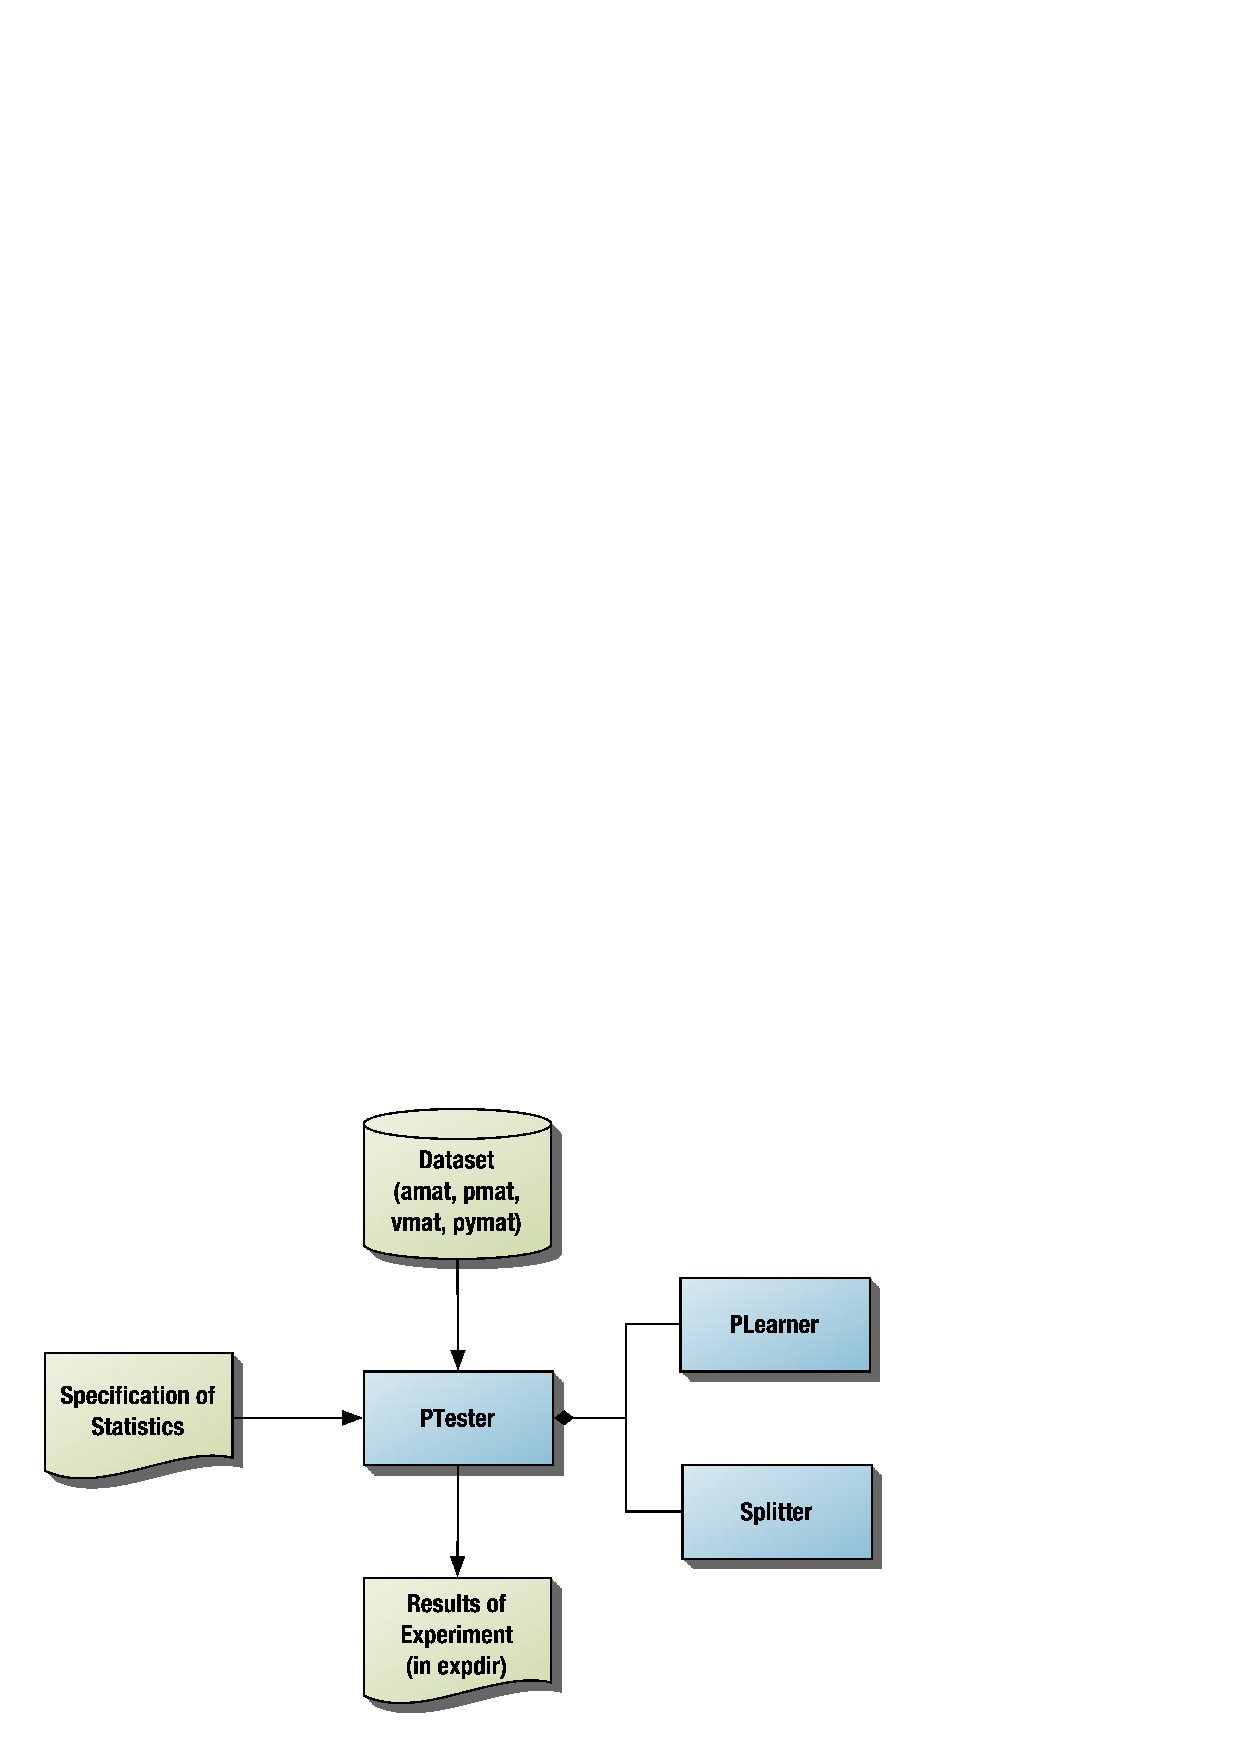
\includegraphics{fig/PTesterOverall.jpg}}
  \caption{Relationship among the classes taking part in the experiment run
    by PTester.  The PLearner must actually be an instance of a class
    derived from PLearner; likewise, the Splitter must be an instance of a
    class derived from Splitter.  The desired statistics are specified as
    options of the PTester object, and the experiment results are stored in
    the experiment directory.}
\label{fig:ptesteroverall}
\end{figure}

\subsection{Process Underlying PTester}

The process underlying PTester is illustrated in
Figure~\ref{fig:ptesterprocess}.

\begin{figure}
  \centering
  \resizebox{0.85\textwidth}{!}{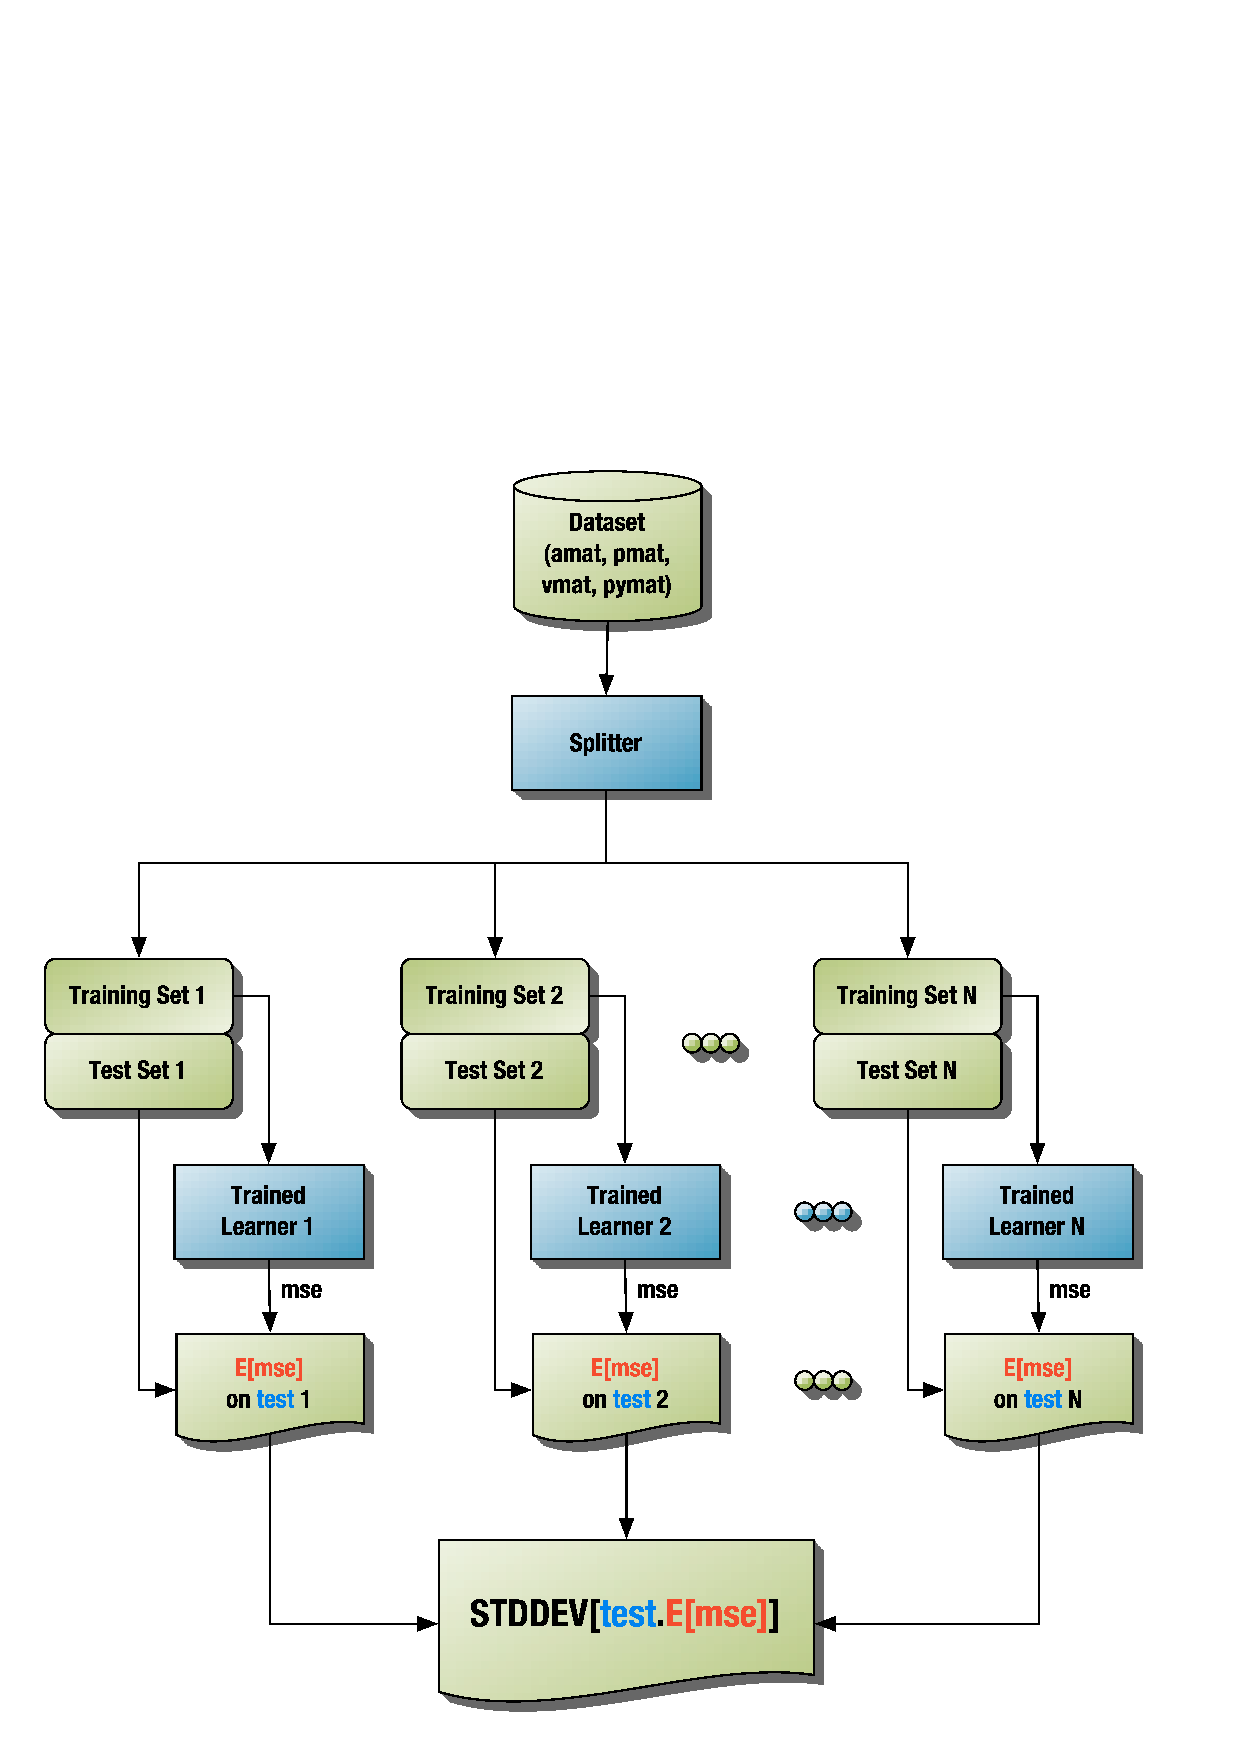
\includegraphics{fig/PTesterProcess.jpg}}
  \caption{Process Underlying PTester}
  \label{fig:ptesterprocess}
\end{figure}

\subsection{Experiment Directory}

\verb|PTester| executes its experiment in a designated \emph{experiment
  directory} (often abbreviated \verb|expdir|, the name of the option used
to specify it within the \verb|PTester| object.)  This directory should be
empty at the beginning of the experiment (if it does not exist, it is
created automatically); if it contains the results of a previous
experiment, \verb|PTester| complains loudly and exits immediately.

Note that if you run your experiments from \verb|.pyplearn| scripts, a
synthetic experiment directory of the form
\verb|expdir_YYYY_MM_DD_HH:MM:SS| is created for you automatically, which
pretty much guarantees uniqueness of the name.

\subsection{Example}

(See the \verb|.pyplearn| tutorial.)

\fi

\section{Python Preprocessing}

See the {\bf pyplearn tutorial}

\chapter{Older Tutorial}

%% author Martin Monperrus

\section{Introduction}

% PLearn is above all a C++ Library for research in the field of Machine
% Learning. But it also comes with a set of tools and programs, that allow
% you to easily carry out experiments.

PLearn is an open source software for machine learning, with numerous features.
It can be used as an runnable software or as a library. This tutorial will help 
you to discover what is PLearn and how to use it.
I assume that:
\begin{itemize}
\item you have basic concepts in machine learning.
\item you have basic concept in object programming.
\item you have a PLearn binary that runs.
\end{itemize}

\section{A basic classification problem}

\subsection{First steps}
We consider the following classification problem. In a 2-D space, we have two 
classes. The problem is represented on figure \ref{classpb}. 

\begin{figure}
  \center{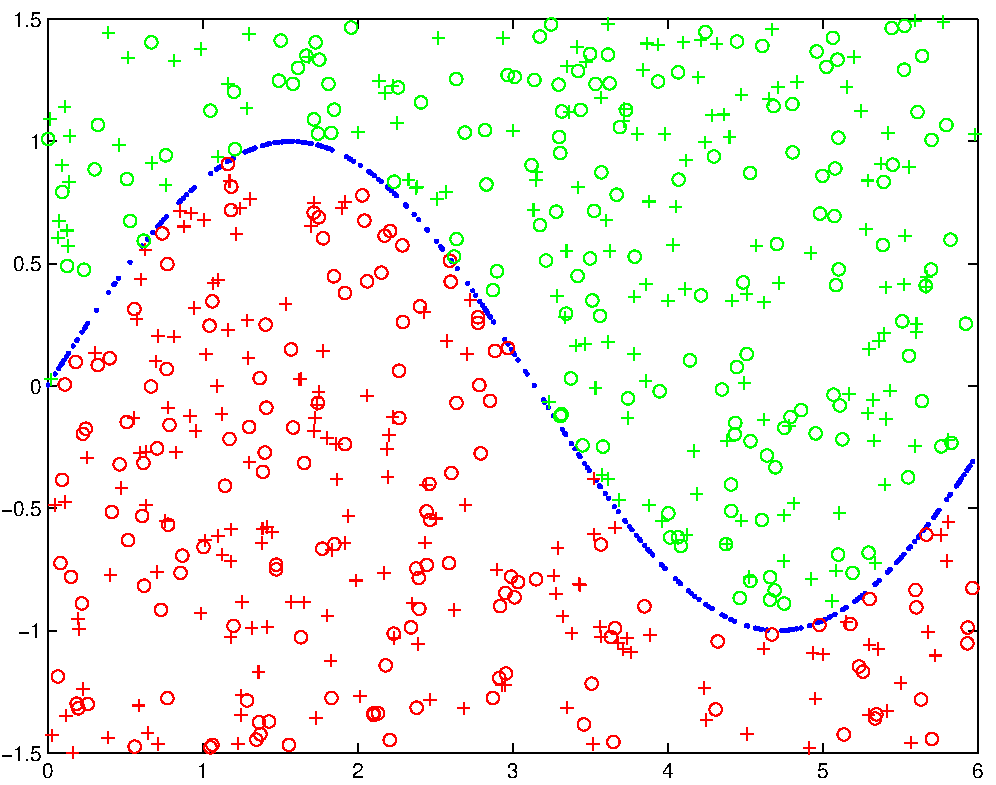
\includegraphics[width=100mm]{Figures/class}}
  \caption{In red, the first class. In green, the second one. In blue, the 
analytic decision boundary. The train examples are 0, the test ones +}  
\label{classpb}
\end{figure}

The data are generated with a Matlab script, called 
task1.m\footnote{provided in \texttt{Plearn/examples}, as all the other sources for this tutorial}.The 
script generates boundary.amat, train.amat, test.amat, and space.amat.
% \verbatiminput{../examples/task1.m}

Now, let's train a neural network on this task with PLearn.

We create the PLearn script, a kind of configuration file:
\verbatiminput{../examples/NNet.plearn}

We call this file \texttt{NNnet.plearn}.

Now we have to specify the dataset. In a classification problem, the dataset is 
a set of examples and their associated classes. We have already created such a 
file in Matlab, called train.amat.
Now we have to specify to PLearn that the two first columns of ``train.amat'' 
contain the data, and the last column the class label, which is in ${-1,1}$, 
corresponding to the output of a tanh.

All this tasks are made with the following file, called \texttt{train.vmat}:
\verbatiminput{../examples/train.vmat}

Now, let's train the network with the folllowing command:

\texttt{plearn learner train NNet.plearn train.vmat final.psave}

Then test on the original space:

\texttt{plearn learner compute\_outputs final.psave space.amat 
out.pmat}

We need two additionnals commands to view the result of the network with matlab:

\texttt{plearn vmat convert out.pmat out.amat} converts from a binary to an ascci file.

\texttt{tail +3 out.amat > result.mat} removes meta-information at the beginning of the file.

Then we execute the result\_task1.m script in Matlab to plot the result, as in figure 
\ref{df}.\begin{figure}
  \center{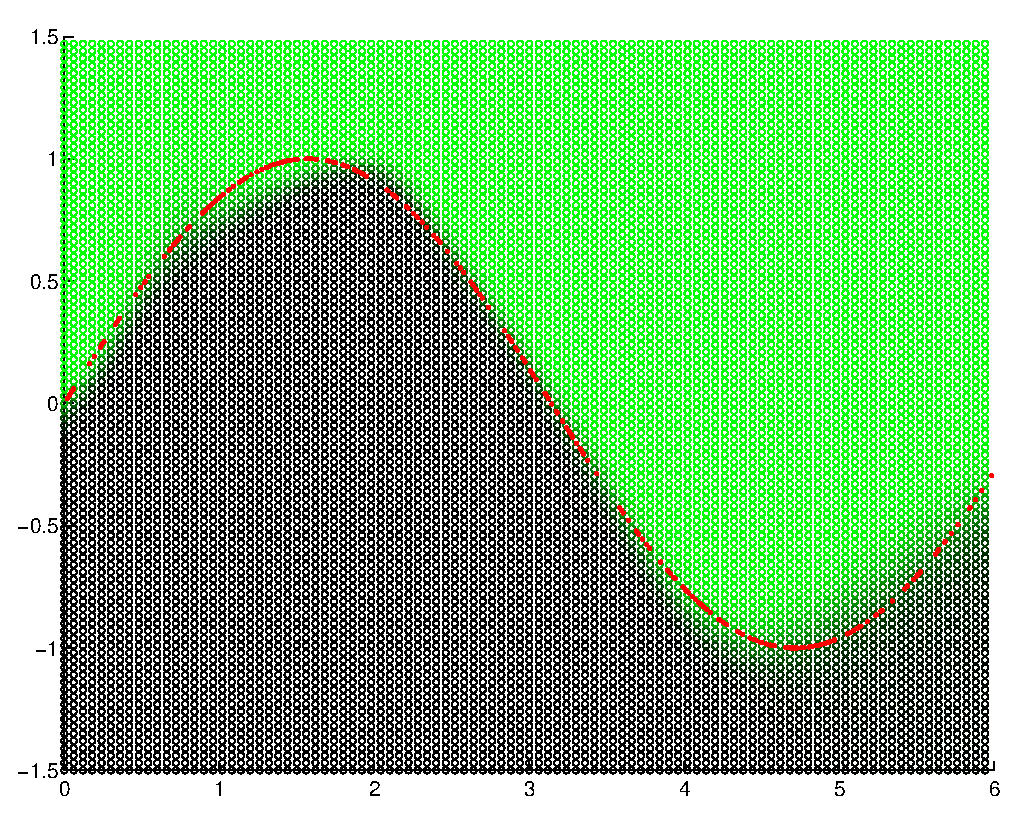
\includegraphics[width=100mm]{Figures/decbound}}
  \caption{Analytic and learned boundary}  
\label{df}
\end{figure}

\subsection{What have we done?}

NNet.plearn contains informations about the neural net. train.vmat contains informations about the the dataset.

PLearn is built with a direct help system. For example:

\texttt{plearn help NNet}

\texttt{plearn help AutoVMatrix}

\texttt{plearn help GradientOptimizer}

This commands gives you an accurate information.

Here are the more important thing about PLearn.

\begin{bf}PLearn is an object oriented software. The scripting language is object 
oriented. ``plearn help NameOfTheClass'' gives you the corresponding information
\end{bf}

Note that a lot of others parameters exist for each classes but they have default values.

\section{A second example}

We now consider a regression problem. We want to train a neural network to predict a sinus.

First, we generate the data with the task2.m matlab file.

Then we perform the task within only one script, the following \texttt{regression.plearn}.

\verbatiminput{../examples/regression.plearn}

Let's run Plearn on this script:
\texttt{plearn regression.plearn}

Then test on the original space:
\texttt{plearn learner compute\_outputs tutorial\_task2/Split0/final\_learner.psave space2.amat out.pmat}

We need two additionnals commands to view the result of the network with matlab:

\texttt{plearn vmat convert out.pmat out.amat}

\texttt{tail +3 out.amat > result.mat}

Let's view the result with a matlab script, result\_task2.m:

\begin{figure}
  \center{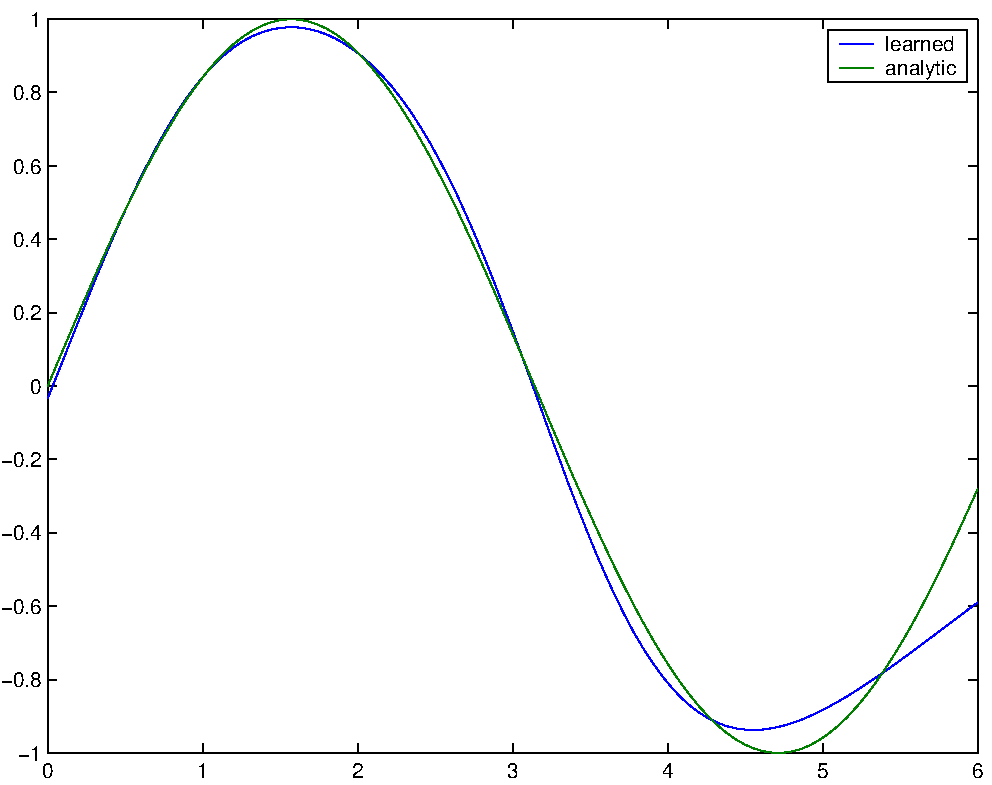
\includegraphics[width=100mm]{Figures/reg}}
  \caption{Analytic and learned function}  
\label{reg}
\end{figure}

\subsection{What have we done?}

We encapsulated the experiment in a powerful scriptable class called ``PTester''.

The command \texttt{plearn help PTester} gives you the corresponding information.
Note that a lot of others parameters exist for PTester but they have default values.

Furthermore, explore all the files that a PTester creates:

\begin{verbatim}
cd tutorial_task2/
ls
plearn vmat view split_stats.pmat
plearn vmat view global_stats.pmat
cd Split0
ls
less test1_stats.psave
less final_learner.psave
\end{verbatim}


\section{Conclusion}
This short tutorial shows a small part of PLearn. Continue by yourself and have a nice Plearn time! 






\chapter{Basics}

\section{The plearn Program}

The {\tt plearn} program is to be found in PLearn/commands and is used to
\begin{itemize}
\item either run a .plearn script 
\item or run a plearn command
\end{itemize}

Plearn scripts are essentially text files ending in .plearn that describe
a learning experiment to be performed.

Plearn commands are typically little tools that allow you to manipulate or examine
datasets or result files, but they can also launch more evolved interactive programs.

The {\tt plearn} program has a simple yet very useful command-line help system.
Type \verb!plearn help! to have an overview.

\section{Essential Commmands}

The basic plearn command is \texttt{plearn script.plearn}.

The wisest command is \texttt{plearn help ClassFoo}.

But there are others:

\texttt{plearn vmat view bidule.vmat} to view any .vmat, .pmat or .amat file.

\texttt{plearn vmat convert truc.pmat truc.amat} to convert a specific data format in an other.

\texttt{plearn learner train}, \texttt{plearn learner test}, \texttt{plearn
  learner computes\_output} provide useful shortcuts to avoid creating long
.plearn script (cf. Tutorial).

If you are interested in more information,

\begin{verbatim}
plearn help commands
plearn help vmat
plearn help learner
\end{verbatim}

\section{Essential Classes}

Here is a list of essential classes.

\begin{verbatim}
plearn help AutoVMatrix
plearn help PTester
plearn help Optimizer
--- plearn help GradientOptimizer
plearn help PLearner
--- plearn help NNet
\end{verbatim}

\section{The .plearn Object File Format}

PLearn uses the same simple file format, both to describe experiments to be
performed (in .plearn scripts), and to save and restore objects
such as a trained neural-network (in .psave or .spec files).

Essentially these files contain the specifications of PLearn objects.

This is a typical .plearn script:

\verbatiminput{../examples/regression.plearn}

Objects are specified by the name of their type, followed by a list of
\verb!option = value! pairs. 

Any sequence of spaces, newlines, tabs, comma, or semicolon is considered a
separator. So colons and semicolons are just there to ease the reading,
spaces would work just as well.

Comments start with a \verb!#! and continue until the end of the line.

The following table sums up the formats that can be used for the values of
an option of a given type

\begin{table}[h]
\caption{ Ascii format for given data-types }
\label{tab:ascii-format-ex}
\begin{tabular}{|l|l|} \hline 
{\bf Data type}         & {\bf Format example} \\ \hline
Any subclass of Object & {\tt ObjectType( option1 = value1, option2 = value2, ... )} \\ \hline
integer                 & {\tt -365} \\ \hline
floating number         & {\tt -3.2e-4} \\ \hline
string                  & {\tt "any string"} \\ \hline
character               & {\tt 'x'} \\ \hline
1D sequences            & {\tt [ 10, 20, 30, 40 ] } \\ 
                        & {\tt [ 10 20 30 40 ] } \\
                        & {\tt 4 [ 10 20 30 40 ] } \\ 
                        & {\tt 4 [ "aa", "bb", "cc", "dd" ] } \\ \hline
2D matrices             & \verb!3 2 [ 1 2  10 20  30 40 ]!    \\ \hline
pairs                   & {\tt 1 : "one" }  \\ \hline
maps                    & \verb!{ 1:"one", 2 :"two", 3: "three" }! \\ \hline
pointers to new object  & \verb!*1 -> ObjType( ... )! \\ \hline
reference to pointer    & \verb!*1;! \\ \hline
\end{tabular}
\begin{center}
\end{center}
\end{table}

Note for strings: unquoted strings, while not recommended are also supported. They are read until
a separator (blank, comma, \ldots) or opening or closing symbol (parenthesis, bracket, \ldots) is met.


\section{The .amat File Format}

Ascii data file.

The new format is as follows:
The size of the matrix is indicated by a line starting with \verb!#size:! and followed by length (number of rows) and width (number of columns)
An optional line starting with \verb!#:! gives the names of the fields (the columns)
Regular comment lines start with a single \verb!#!.

ex:

\begin{verbatim}
# Characteristics of a population of 534
#size: 534 3
#:  age height weight
     33  1.72   71
    25  1.80   80
\end{verbatim}

\section{The .pmat File Format}

PLearn native binary format.

\section{The .vmat File Format}

File containing a description of a virtual dataset.

A .vmat is a text specification of a dataset built from the composition of source data, possibly with operations applied to it.

\verbatiminput{../examples/train.vmat} 

% This is not a NO-Lisa information

% \section{Preprogrammed datasets}
% 
% \begin{itemize}
% \item 2d
% \item letters -> Letter Image Recognition data
% \item breast -> The Wisconsin Breast Cancer problem
% \item usps
% \item mnist
% \end{itemize}


\chapter{Howto}

\section{How to Build a Neural Network?}

You should have learned with the tutorial basic PLearn neural network. The class used is NNet.

Here is a basic NNet script object:

\verbatiminput{../examples/BasicNNet.spec}


% ------------------------------------------------------------------------------------------
% ------------------------------------------------------------------------------------------
\chapter{Advanced}
% ------------------------------------------------------------------------------------------
% ------------------------------------------------------------------------------------------

\section{The .sdb File Format}

Any simpledb can be automatically seen as a numeric vmat dataset. 
String fields are removed.

\section{The .dmat/ Format }

Directory containing compressed data.

Contains:
\begin{itemize}
\item 0.data, 1.data, 2.data
\item indexfile
\item fieldnames
\end{itemize}

\section{Advanced .vmat}

The description is made through a set of sections (all optional except SOURCES) enclosed in xml-like tags.

There is a program named vmat (although it handles many dataset formats) that can be used to perform useful tasks with datasets. Two of them are relevant here. 

Calling \verb!vmat gendef datasetname 10 20! will first generate a stats.def file in the metadata directory of the dataset containing a define for each field for each supported statistic. Then it will generate files bins10.def and bins20.def containing defines that can be used to bin the fields (with 10 and 20 bins). These defines can then be used (with INCLUDE) in the VPL code.

Use \verb!vmat genvmat datasetname (binned\{num\} | onehot\{num\} | normalized)! to generate automatically a vmat that will do the same operation on all fields.

Here's an example of a .vmat file:
\begin{verbatim}
<SOURCES>
/u/Gaston/some_source.amat /u/Gaston/some_source3.sdb
</SOURCES>

<PREFILTER>
INCLUDE /u/Gaston/some_source.amat.metadata/stats.def
@some_field @some_field.mean >=
</PREFILTER>

# this is a comment

<JOIN>
/u/jkeable/PLearn/UserExp/jkeable/joinVMatrix/slave.amat
[id,val] == [id,val1]
MEAN(claim) :claim.mean
</JOIN>

<PROCESSING>
%0 %1 + :my_sum
# this is another comment
[%2:@claim.mean]
</PROCESSING>

<POSTFILTER>
@claim.mean isnan not
</POSTFILTER>

<SIZES>
100
1
0
</SIZES>

<PRECOMPUTE> dmat </PRECOMPUTE>
\end{verbatim}


\subsection{SOURCES}
The SOURCES section is the only one that is not optional. It describes the source dataset(s) (in any format) that the vmat will be built from. In its most complex form, the syntax of the specification is a matrix of NxM dataset strings. The datasets are first concatenated horizontally, then vertically. Thus, all datasets on a same row must have the same length, and the results of all horizontal concatenation, the same width.

\subsection{PREFILTER and POSTFILTER}

Those sections are use to perform filtering at different stages of the vmat construction. Prefiltering is made after processing of the SOURCES section, while the postfiltering is made after the JOIN and PROCESSING section are executed. 

The syntax of the filtering operations is VPL, which is a postfix language described further down. After execution of the code, a value must remain on the execution stack. If it non zero, the row will be kept, otherwise, it is rejected.

\subsection{JOIN}

This section is used to perform a pseudo-join operation between a master and a slave table. At this time, a standard join operation (cartesian product) is not possible. Instead, slave rows matching a master row are used to compute statistics appended to the master row. The syntax is:

\begin{verbatim}
slave_dataset
[master_field1,...,master_fieldN] == [slave_field1,...,slave_fieldN]
STATISTIC1(slavefield1) :newfield_name1
STATISTIC2(slavefield2) :newfield_name2
...
\end{verbatim}
where STATISTIC is one of: {COUNT | NNONMISSING | NMISSING | SUM | SUMSQUARE | MEAN | VARIANCE | STDDEV | STDERR | MIN | MAX}. 

Note that you can repeat the operation multiple times in a single JOIN section.

\subsection{PROCESSING}
Use this section to modify or create new fields in the dataset (e.g: binning operations, onehot conversions, etc..). The processing is specified with VPL, described later.

As soon as you declare a PROCESSING section, all fields resulting from previous operations (sources concatenation, join operations) are not included automatically in the resulting matrix (obviously, you can still refer to them), so it is empty unless you declare them manually. In the small example given above, the operations done are the replacement of the first two fields by their sum, and then the remaining fields are appended in the resulting matrix with the second line. See VPL section for more details.

\subsection{SIZES}
This section lets you define the input size, target size and weight size of the matrix.
They must be given in this specificic order, each on one line.
This is especially useful when the .vmat file is loaded through an AutoVMatrix for instance, so
you don't have to specify the sizes in the AutoVMatrix itself.

\subsection{PRECOMPUTE}
When you need speed, use this section to create a precomputed version of you vmat. This version will be computed the first time the vmat is loaded. You specify the type of file you want the precomputed version to be saved to (dmat or pmat). See example above.

The synchronization of the precomputed version is ensured through an almost-intelligent mechanism that checks the date of sources recursively. Note: we decided that include files (e.g: statistics) that are out of date issue a warning, but will not force recomputation. This could be changed. 

\subsection{DEBUG}
Including this section will force output of preprocessed VPL to stderr.

\subsection{The VPL language}
VPL (vmat processing language) is a home brewed mini-language in postfix notation. As of today, it is used is the \{PRE,POST\}FILT\-ERING and PROCESSING sections of a .vmat file. It supports INCLUDEs instructions and DEFINEs (dumb named string constants). It can handle reals as well as dates (format is: CYYMMDD, where C is 0 (1900-1999) or 1 (2000-2099). The language will not be extensively described here. For more info, you can look at
plearn/vmat/VMatLanguage.*. 

A VPL code snippet is always applied to the row of a VMatrix, and can only refer to data of that row. The result of the execution will be a vector, which is the execution stack at code termination. 

When you use VPL in a PROCESSING section, each field you declare must have its associated fieldname declaration. The compiler will ensure that the size of the result vector and the number of declared fieldnames match. This doesn't apply in the filtering sections since the result is always a single value. 

To declare a fieldname, use a colon with the name immediately after. To batch-declare fieldnames, use eg.:myfield:1:10. This will declare fields myfield1 up to myfield10.

There are two notations to refer to a field value: the @ symbol followed by the fieldname, or \% followed by the field number.

To batch-copy fields, use the following syntax: [field1:fieldn] (fields can be in @ or \% notation).

Here's a real-life example of a PROCESSING section:

\begin{verbatim}
<PROCESSING>
@lease_indicator 88 == 1 0 ifelse :lease_indicator
@rate_class 1 - 7 onehot :rate_class:0:6
@collision_deductible { 2->1; 4->2; 5->3; 6->4; 7->5; 
[8 8]->6; MISSING->0; OTHER->0 }
7 onehot :collision_deductible:0:6
@roadstar_indicator 89 == 1 0 ifelse :roadstar_indicator
</PROCESSING>
\end{verbatim}

\section{The Metadata Directory}

A metadata directory is associated with each dataset.  For the datasets
corresponding to a file ({\tt .amat, .pmat, .vmat}) or directory ({\tt .dmat/}) the
associated metadata directory is obtained by appending {\tt .metadata/} to the
file or directory name.

A metadata directory will typically contain the following cache directories to avoid recomputing costly things

\begin{itemize}
\item \verb!STATSCACHE/! contains cached statistics
\item \verb!MODELCACHE/<classname>/! contains any pertinent cached data computed on this dataset by objects of class \verb!<classname>!
\end{itemize}

In addition, the {\tt .metadata} directory associated with a {\tt .vmat} may contain
\begin{itemize}
\item {\tt precomputed.dmat/} or {\tt precomputed.pmat} if the {\tt .vmat} description specified \verb!<PRECOMPUTE>!
\item {\tt source.index} containing row indexes in the source (resulting from \verb!<PREFILTER>!, \verb!<POSTFILTER>!, \verb!<SHUFFLE>!)
\end{itemize}



\chapter{Appendix A: File Formats}

\section{The .plearn and .psave Formats}

\subsection{Generalities on mixing ascii and binary}

The following characters are in many cases skipped before reading any
element: space, tab, newline, carriage-return, comma and semicolon. They
are essentially ignored. Binary serialized things should always start with
a non-printable ascii character.


\subsection{TVec and TMat}

TVec and TMat will be serialized differently depending on the {\em
implicit\_storage} flag of the PStream they are being written to.

If {\em implicit\_storage} is set, then serialization won't write the actual
whole structure of the TVec or TMat, but will only save the size information
and elements as a 1D or 2D {\em sequence} (see \ref{ascii-sequence} and
\ref{binary-sequence}), ex:

\begin{verbatim}
4 [ 1.2 3.5 2.8 5.2 ]

3 2 [
0.1    0.2
0.3    0.4
0.5    0.6
]
\end{verbatim}

If {\em implicit\_storage} is false, then the complete structure of the
TVec or TMat with the pointer to its storage (possibly shared with others)
will be written explicitly. This corresponds to true, deep serialization.

Ex:

\begin{verbatim}
TVec( 4 0 
*1->Storage(4 [ 1.2 3.5 2.8 5.2 ]) )

TMat( 3 2 2 0 
*2->Storage(6 [ 0.1 0.2 0.3 0.4 0.5 0.6 ] ) )
\end{verbatim}

For TVec, we have {\em length offset} followed by the storage pointer.
For TMat, we have {\em length width mod offset} followed by the storage pointer.

This allows to keep structure. For example, if we had a submatrix viewing
the second column of the previous TMat, we would have:

\begin{verbatim}
TMat( 3 1 2 1
*2 )
\end{verbatim}

\subsection{Binary PLearn format for base types}

To allow mixing of ascii and binary in a file, a non-printable ascii
character is used as a one-byte header to identify any binary portion.  In
Table~\ref{tab:base-types} we give the header codes for all basic types

Note that char is considered to be the same as signed char, and long is
considered to be the same as int, i.e.: 4-bytes long, which is the case on
current architectures.

\begin{table}[h]
\caption{ Binary-header codes for base types }
\label{tab:base-types}
\begin{tabular}{|llcl|} \hline 
Base type      & Byte order    & Header byte & Number of bytes to follow \\ \hline 
char           & -             & 0x01        & 1 \\
signed char    & -             & 0x01        & 1 \\
unsigned char  & -             & 0x02        & 1 \\
short          & little-endian & 0x03        & 2 \\
short          & big-endian    & 0x04        & 2 \\
unsigned short & little-endian & 0x05        & 2 \\
unsigned short & big-endian    & 0x06        & 2 \\
int            & little-endian & 0x07        & 4 \\
int            & big-endian    & 0x08        & 4 \\
unsigned int   & little-endian & 0x0B        & 4 \\
unsigned int   & big-endian    & 0x0C        & 4 \\
long           & little-endian & 0x07        & 4 \\
long           & big-endian    & 0x08        & 4 \\
unsigned long  & little-endian & 0x0B        & 4 \\
unsigned long  & big-endian    & 0x0C        & 4 \\
float          & little-endian & 0x0E        & 4 \\
float          & big-endian    & 0x0F        & 4 \\
double         & little-endian & 0x10        & 8 \\
double         & big-endian    & 0x11        & 8 \\ \hline 
PRInt64        & little-endian & 0x16        & 4 \\
PRInt64        & big-endian    & 0x17        & 4 \\
PRUint64       & little-endian & 0x18        & 4 \\
PRUint64       & big-endian    & 0x19        & 4 \\
\end{tabular}
\begin{center}
\end{center}
\end{table}

\begin{itemize}
\item booleans are represented the same way in binary mode as in ascii mode: with the character 0 (for false) or 1 (for true). There is no header byte.
\item C++ pairs are indicated by a header-byte 0x16 followed by serialization of the two elements.
\end{itemize}


\subsection{Ascii PLearn format for a sequence}
\label{ascii-sequence}

We consider both one-dimensional sequences ( array, vector, \ldots) which only have a length,
and two-dimensional sequences which have a length and a width.

Ascii-serialized one-dimensional sequences will have the following format:

{\em length} \verb{[ ... ... ... ]{

with the elements of the sequence separated by a single space.

However, on reading, several variations of this format are recognized:
\begin{itemize}
\item The elements may be separated by any number of blanks (space, tab, newline) and/or commas or semicolons.
\item The {\em length} may be omitted
\end{itemize}

Ascii-serialized two-dimensional sequences will have the following format:

{\em length} {\em width} {\tt [} 
\begin{verbatim}
... ... ...
... ... ... 
]
\end{verbatim}

with the elements of each row separated by a tab, and the rows separated by a newline.

However on reading, blanks, commas and semi-colons between elements are
completely ignored (skipped), so you may format the data as you wish.

2D Sequences are used exclusively for TMats.
Notice that it's also possible to make a 1D sequence of 1D sequences, but that's different from a 2D sequence.

\subsection{Binary PLearn format for a sequence}
\label{binary-sequence}

We consider both one-dimensional sequences ( array, vector, \ldots) which only have a length,
and two-dimensional sequences which have a length and a width.

The following table gives the corresponding header-byte:

\begin{tabular}{|lll|} \hline
Type of sequence & byte-order    & Header byte \\ \hline
one-dimensional  & little-endian & 0x12        \\ 
one-dimensional  & big-endian    & 0x13        \\ 
two-dimensional  & little-endian & 0x14        \\ 
two-dimensional  & big-endian    & 0x15        \\ \hline
\end{tabular}

All that follows is supposed to be in the byte-order implied by the header-byte.

The first header-byte is followed by an {\em element-type} byte giving the nature
of the elements in the sequence.  It can be either the byte identifying a
base-type given in Table~\ref{tab:base-types} (the endianness must match),
or {\tt '0' = 0x30} to indicate a sequence of booleans (1 byte per boolean) 
or {\tt 0xFF} to indicate a {\em generic} sequence.

The header bytes are followed by one (for 1D sequences) or two (for 2D)
4-byte int to indicate the length (and possibly width) of the sequence.
So the total header size for sequences is 6 bytes for 1D sequences and 10
bytes for 2D sequences.

This header is followed by a dump of the elements of the sequence (in
row-major mode for 2D).  Notice that a sequence of a base type, may be
saved as a {\em generic} sequence (with the {\em element-type} byte {\tt 0xFF})



\begin{tabular}{|l|l|l|} \hline
Type of sequence         & Header byte & Followed by \\ \hline
Generic on little-endian & 0x12        & size as 4-byte little-endian int, \\
                         &             & then binary serialization of the elements \\ \hline
Generic on big-endian    & 0x13        & size as 4-byte big-endian int, \\ 
                         &             & then binary serialization of the elements \\ \hline
Sequence of a base-type  & 0x14        & size as 4-byte little-endian int, \\ 
on little-endian         &             & base-type given by header byte in previous \\
                         &             & table, followed by binary dump of elements \\ \hline
Sequence of a base-type  & 0x15        & size as 4-byte big-endian int, \\ 
on big-endian            &             & base-type given by header byte in previous \\
                         &             & table, followed by binary dump of elements \\ \hline
\end{tabular}





\chapter{(DEPRECATED) Directory and file structure for old experiments}

This is the structure with the old experiment system. And it's deprecated. 

\begin{verbatim}
/home/exp/<project>/<task>/
  - dataset.aliases
  - model.aliases
   
.../modelalias/
  # for normal train/test
  <trainalias>.<testalias>.results
  <trainalias>.psave                   # best model so far
  <trainalias>.epoch<epoch>.psave
  <trainalias>.epoch<epoch>.<testalias>.outputs
  <trainalias>.epoch<epoch>.<testalias>.costs

  # For bootstrap ( <i> is the index of the trainset variant )
  <trainalias>.bs_<bsparams>_<i>.<testalias>.results
  <trainalias>.bs_<bsparams>.testalias.results.summary
  <trainalias>.bs_<bsparams>_<i>.psave   # best model so far
  <trainalias>.bs_<bsparams>_<i>.epoch<epoch>.psave
  <trainalias>.bs_<bsparams>_<i>.epoch<epoch>.<testalias>.outputs
  <trainalias>.bs_<bsparams>_<i>.epoch<epoch>.<testalias>.costs

  # For k-fold  ( <i> is the index of the trainset variant )
  <trainalias>.kf_<k>_<i>.<testalias>.results
  <trainalias>.kf_<k>.testalias.results.summary
  <trainalias>.kf_<k>_<i>.psave   # best model so far
  <trainalias>.kf_<k>_<i>.epoch<epoch>.psave
  <trainalias>.kf_<k>_<i>.epoch<epoch>.<testalias>.outputs
  <trainalias>.kf_<k>_<i>.epoch<epoch>.<testalias>.costs
  
  # For sequential validation  ( <i> is the index of the trainset variant )
  <trainalias>.sv_<svparams>_<i>.<testalias>.results
  <trainalias>.sv_<svparams>.testalias.results.summary
  <trainalias>.sv_<svparams>_<i>.psave   # best model so far
  <trainalias>.sv_<svparams>_<i>.epoch<epoch>.psave
  <trainalias>.sv_<svparams>_<i>.epoch<epoch>.<testalias>.outputs
  <trainalias>.sv_<svparams>_<i>.epoch<epoch>.<testalias>.costs
\end{verbatim}

And from the old\_plearn command....:

\begin{verbatim}
The 'plearn' program is designed to strongly encourage the following
directory and file structure for carrying experiments.  Suppose we have a
root "experiment" directory, EXP, that is to contain all the results of all
the experiments on all projects ever carried.

Here is the recommended structure:

EXP/PROJECT/TASK/DATA-REPRESENTATION/MODELALIAS
|___________________________________|
                 |
            SPECDIR (will typically contain 'dataset.aliases', specifying datasets 
                                            and 'model.aliases' specifying learners with learneroptions)

PROJECT is the name of the higher level project, regarding a particular set

TASK should represent a particular learning task for which you wish to
     assess different methods (ex: condprob_of_claim)

DATA-REPRESENTATION is the notion of using different data representations
                    (to suit underlying learner) for a task. (ex:
                    onehot_inputs_integer_target)

The directory organization down to DATA-REPRESENTATION is only
indicative. You may name the directories as you please (including the
DATA-REPRESENTATION directory), add or omit hierarchy levels, etc...

The organization below DATA-REPRESENTATION is however enforced by the
'plearn' program.  DATA-REPRESENTATION *must* contain a 'dataset.aliases'
file defining the datasets to be used (in that representation). Everything
below DATA-REPRESENTATION will use those datasets. 

Because it contains the actual dataset specification in dataset.aliases 
and models specifications in model.aliases
we also call EXP/PROJECT/TASK/DATA-REPRESENTATION/
             |___________________________________|
                              |
                           SPECDIR

Ex of dataset.aliases file:
train /home/db/finance/stock3proj/discreterepr_trainset
valid /home/db/finance/stock3proj/discreterepr_testset1
test /home/db/finance/stock3proj/discreterepr_testset2

An alias for 'train' is mandatory. You can give aliases to any number of
other datasets ('valid' and 'test' are customary but you could also use
'test1' 'testsomemore' 'strangetestset' etc...)
The actual dataset specification can be any string understood by getDataSet.


The model.aliases file should contain one line for each
learnertype+learnerparams you are considering. The line starts for an
'alias' for that particular learnertype+learnerparams combination. That
alias, which will also be the name of its result directory, must be
followed by a learner classname, and a semi-column separated string of
options of the form optionname=optionvalue, in the format understood by
that learner's setOption method.

Formally, that is: 
<alias> <classname> <option1=...; option2=...; ...>
ex: knn5 KNN inputsize=210; k=5 

The following files will typically be created consequently by the 'plearn' program
in the corresponding <alias> directory.

- train.objective   
  Ascii file reporting the cost as it is optimized by the learner (and other possible costs)
- model#.psave        
  Contains the saved model (at 'epoch' #, see below).
- <datasetalias>.results 
  Ascii file reporting the average costs achieved by the model on the 
  specified dataset (also includes stderr, min, max of those costs)
- model#.<datasetalias>.outputs.pmat 
  The individual outputs of the model obtained on the specified dataset
- model#.<datasetalias>.costs.pmat
  The individual costs of the model obtained on the specified dataset

For learners performing iterative optimization (or some form of incremental
learning) and able to save and test intermediate models, the # stands for
the 'epoch' number of the model saved (starting at 0).  It will also
correspond to the data-row number in train.objective and
<datasetalias>.results
\end{verbatim}


\chapter*{License}

This document is covered by the license appearing after the title page.

\vspace*{.5cm}

The PLearn software library and tools described in this document are
distributed under the following BSD-type license:

\begin{verbatim}
Redistribution and use in source and binary forms, with or without
modification, are permitted provided that the following conditions are met:
 
  1. Redistributions of source code must retain the above copyright
     notice, this list of conditions and the following disclaimer.
 
  2. Redistributions in binary form must reproduce the above copyright
     notice, this list of conditions and the following disclaimer in the
     documentation and/or other materials provided with the distribution.
 
  3. The name of the authors may not be used to endorse or promote
     products derived from this software without specific prior written
     permission.
 
 THIS SOFTWARE IS PROVIDED BY THE AUTHORS ``AS IS'' AND ANY EXPRESS OR
 IMPLIED WARRANTIES, INCLUDING, BUT NOT LIMITED TO, THE IMPLIED WARRANTIES
 OF MERCHANTABILITY AND FITNESS FOR A PARTICULAR PURPOSE ARE DISCLAIMED. IN
 NO EVENT SHALL THE AUTHORS BE LIABLE FOR ANY DIRECT, INDIRECT, INCIDENTAL,
 SPECIAL, EXEMPLARY, OR CONSEQUENTIAL DAMAGES (INCLUDING, BUT NOT LIMITED
 TO, PROCUREMENT OF SUBSTITUTE GOODS OR SERVICES; LOSS OF USE, DATA, OR
 PROFITS; OR BUSINESS INTERRUPTION) HOWEVER CAUSED AND ON ANY THEORY OF
 LIABILITY, WHETHER IN CONTRACT, STRICT LIABILITY, OR TORT (INCLUDING
 NEGLIGENCE OR OTHERWISE) ARISING IN ANY WAY OUT OF THE USE OF THIS
 SOFTWARE, EVEN IF ADVISED OF THE POSSIBILITY OF SUCH DAMAGE.
\end{verbatim}

\end{document}
